\documentclass[12pt,a4paper,twoside]{report}
% -------------------------------------------------------------------- %
% Pacotes

\usepackage[utf8]{inputenc}
\usepackage[T1]{fontenc}
\usepackage[brazil]{babel}
\usepackage[fixlanguage]{babelbib}
\usepackage[pdftex]{graphicx}      % usamos arquivos pdf/png como figuras
\usepackage{setspace}              % espaçamento flexvel
\usepackage{indentfirst}           % indentação do primeiro parágrafo
\usepackage{makeidx}               % índice remissivo
\usepackage[nottoc]{tocbibind}     % acrescentamos a bibliografia/indice/conteudo no Table of Contents
\usepackage{courier}               % usa o Adobe Courier no lugar de Computer Modern Typewriter
\usepackage{type1cm}               % fontes realmente escaláveis
\usepackage{titletoc}
\usepackage{ucs}
\usepackage[font=small,format=plain,labelfont=bf,up,textfont=it,up]{caption}
\usepackage[usenames,svgnames,dvipsnames]{xcolor}
\usepackage[a4paper,top=2.54cm,bottom=2.0cm,left=2.0cm,right=2.54cm]{geometry} % margens
\usepackage{amsmath}
\usepackage{booktabs} % cria tabelas em formato profissional
\usepackage[pdftex,plainpages=false,pdfpagelabels,pagebackref,colorlinks=true,citecolor=DarkGreen,
linkcolor=NavyBlue,urlcolor=DarkRed,filecolor=green,bookmarksopen=true]{hyperref} % links coloridos
\usepackage[all]{hypcap}                % soluciona o problema com o hyperref e capítulos
\usepackage[square,sort,nonamebreak,comma]{natbib}  % citação bibliográfica alpha
\fontsize{60}{62}\usefont{OT1}{cmr}{m}{n}{\selectfont}
\usepackage{upquote}                    % formata apóstrofes '
\usepackage{textcomp}

% Para formatar corretamente as URLs
\usepackage{url}
% -------------------------------------------------------------------- %
% Cabeçalhos similares ao TAOCP de Donald E. Knuth
\usepackage{fancyhdr}
\pagestyle{fancy}
\fancyhf{}
\renewcommand{\chaptermark}[1]{\markboth{\MakeUppercase{#1}}{}}
\renewcommand{\sectionmark}[1]{\markright{\MakeUppercase{#1}}{}}
\renewcommand{\headrulewidth}{0pt}

\frenchspacing                     % arruma o espaço: id est (i.e.) e exempli gratia (e.g.)
\urlstyle{same}                    % URL com o mesmo estilo do texto e no mono-spaced
\makeindex                         % para o índice remissivo
\raggedbottom                      % para no permitir espaços extras no texto
\fontsize{60}{62}\usefont{OT1}{cmr}{m}{n}{\selectfont}
\cleardoublepage
\normalsize

% -------------------------------------------------------------------- %
% Cores para formatação de código
\usepackage{color}
\definecolor{vermelho}{rgb}{0.6,0,0} % para strings
\definecolor{verde}{rgb}{0.25,0.5,0.35} % para comentários
\definecolor{roxo}{rgb}{0.5,0,0.35} % para palavras-chaves
\definecolor{azul}{rgb}{0.25,0.35,0.75} % para strings
\definecolor{cinza-claro}{gray}{0.95}
% -------------------------------------------------------------------- %
% Opções de listagem usados para o código fonte
% Ref: http://en.wikibooks.org/wiki/LaTeX/Packages/Listings
\usepackage{listings}           % para formatar código-fonte (ex. em Java)

\lstset{ %
language=Python,                      % seleciona a linguagem do código
basicstyle=\footnotesize\ttfamily,    % o tamanho da fonte usado no código
commentstyle=\color{verde}\bfseries,  % formatação de comentários
stringstyle=\color{azul},             % formatação de strings
upquote=true,
numbers=left,                   % onde colocar os números de linha
numberstyle=\tiny,  % o tamanho da fonte usada para a numeração das linhas
stepnumber=1,                   % o intervalo entre dois números de linhas. Se for 1, numera cada uma.
numbersep=5pt,                  % how far the line-numbers are from the code
showspaces=false,               % show spaces adding particular underscores
showstringspaces=false,         % underline spaces within strings
showtabs=false,                 % show tabs within strings adding particular underscores
keywordstyle=\color{roxo}\bfseries,
keywordstyle=[1]\color{roxo}\bfseries,
keywordstyle=[2]\color{verde}\bfseries,
frame=b,                   % adds a frame around the code
framerule=0.6pt,
tabsize=2,                      % sets default tabsize to 2 spaces
captionpos=t,                   % sets the caption-position to top
breaklines=true,                % sets automatic line breaking
breakatwhitespace=false,        % sets if automatic breaks should only happen at whitespace
escapeinside={\%*}{*)},         % if you want to add a comment within your code
backgroundcolor=\color[rgb]{1.0,1.0,1.0}, % choose the background color.
rulecolor=\color[rgb]{0.8,0.8,0.8},
extendedchars=true,
xleftmargin=10pt,
xrightmargin=10pt,
framexleftmargin=10pt,
framexrightmargin=10pt,
literate={â}{{\^{a}}}1  % para formatar corretamente os acentos do Português ao usar utf8
    {ê}{{\^{e}}}1
    {ô}{{\^{o}}}1
    {Â}{{\^{A}}}1
    {Ê}{{\^{E}}}1
    {Ô}{{\^{O}}}1
    {á}{{\'{a}}}1
    {é}{{\'{e}}}1
    {í}{{\'{i}}}1
    {ó}{{\'{o}}}1
    {ú}{{\'{u}}}1
    {Á}{{\'{A}}}1
    {É}{{\'{E}}}1
    {Í}{{\'{I}}}1
    {Ó}{{\'{O}}}1
    {Ú}{{\'{U}}}1
    {à}{{\`{a}}}1
    {À}{{\`{A}}}1
    {ã}{{\~{a}}}1
    {õ}{{\~{o}}}1
    {Ã}{{\~{A}}}1
    {Õ}{{\~{O}}}1
    {ç}{{\c{c}}}1
    {Ç}{{\c{C}}}1
    {ü}{{\"u}}1
    {Ü}{{\"U}}1
}

\renewcommand{\lstlistingname}{Listagem}
\renewcommand{\lstlistlistingname}{Lista de Listagens}

% \captionsetup[lstlisting]{singlelinecheck=false, labelfont={blue}, textfont={blue}}
\usepackage{caption}
\DeclareCaptionFont{white}{\color{white}}
\DeclareCaptionFormat{listing}{\colorbox[cmyk]{0.43, 0.35, 0.35,0.01}{\parbox{\textwidth}{\hspace{15pt}#1#2#3}}}
\captionsetup[lstlisting]{format=listing,labelfont=white,textfont=white, singlelinecheck=false, margin=0pt, font={bf,footnotesize}}

\title{Análise experimental de algoritmos usando Python}
\author{Patricia Mariana Ramos Marcolino\\
\texttt{\small \url{pmrmarcolino@hotmail.com}}
\vspace{1cm} \\
Eduardo Pinheiro Barbosa \\
\texttt{\small \url{eduardptu@hotmail.com}}
\vspace{1cm} \\
Faculdade de Computação \\
Universidade Federal de Uberlândia
}
\date{\today}

\begin{document}
\maketitle
% -------------------------------------------------------------------- %
% Listas de figuras, tabelas e códigos criadas automaticamente
\listoffigures
\listoftables
\lstlistoflistings
% -------------------------------------------------------------------- %

% -------------------------------------------------------------------- %
% Sumário
\tableofcontents
% cabeçalho para as páginas de todos os capítulos
\fancyhead[RE,LO]{\thesection}

%\singlespacing              % espaçamento simples
\setlength{\parskip}{0.15in} % espaçamento entre paragráfos

\chapter{Análise}
\subsection{Introdução}
O bubblesort ou método da bolha, é um algoritmo de ordenação bastante simples, onde comparam-se dois elementos e trocam-se suas posições se o segundo elemento é menor do que o  primeiro. Nesse algoritmo são feitas várias passagens pelo vetor comparando dois elementos adjacentes, se esses elementos estiverem fora de ordem, eles são trocados.\\
Vantagens:\\
    Simplicidade do algoritmo, estável
Desvantagens:\\
    Lentidão\\
Indicações:\\
    Vetores pequenos, demonstrações didaticas

\subsection{Desempenho do bubblesort}
As operações de comparação e de troca de po de elementos são executadas ni pior caso, o algoritmos realizará n-1 troca para o primeiro passo, e depois n-2 trocas para o segundo elemento e assim sucessivamente. Trocas = n-1+n-2+n-2+...+2+1 aproximadamente $n^2$
trocas. No melhor caso nenhuma troca será realizada, pois em ambos os casos o algoritmo faz da ordem, portanto:\\
Complexidade de espaço: o algoritmo tem complexidade de espaço referente ao tamanho do vetor de dados.\\
Complexidade de tempo: tem maior custo em comparações e troca de posições, assim a complexidades de tempo é
\[T(n) = O(n^2)\] 


\chapter{Resultados}
\section{Tabelas}

\begin{table}[ht]
\centering
\begin{tabular}{rrr} \toprule
        n &    comparações &       tempo(s) \\ \midrule
      32  &            496 &      0.000966 \\
      64  &           2016 &      0.004182 \\
     128  &           8128 &      0.014954 \\
     256  &          32640 &      0.061451 \\
     512  &         130816 &      0.236011 \\
    1024  &         523776 &      1.053630 \\
    2048  &        2096128 &      4.185620 \\
    4096  &        8386560 &     16.159700 \\
    8192  &       33550336 &     63.593300 \\
\bottomrule\addlinespace
\end{tabular}
\caption{Tabela com vetor teste aleatório: a linha de interesse analisada para este caso é a 15}
\label{tab:bolhaAleatorio}
\end{table}


\begin{figure}[ht]
\centering 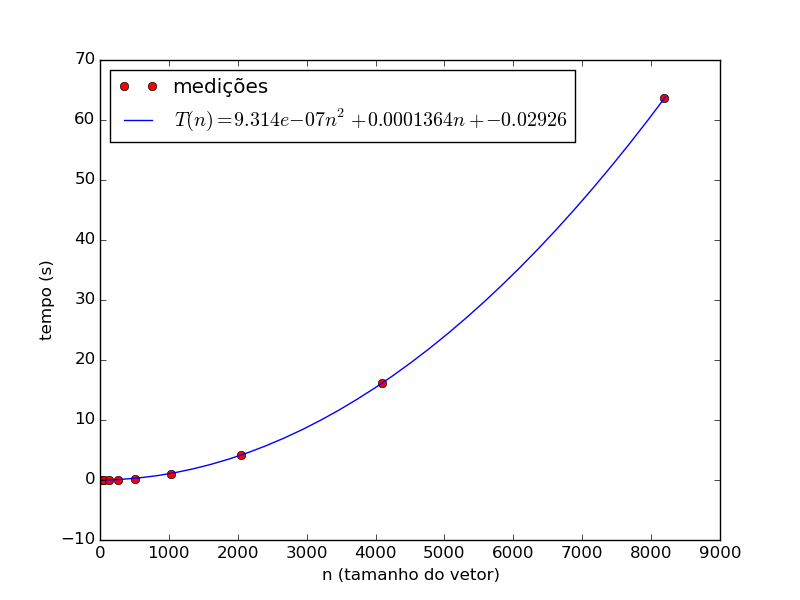
\includegraphics[scale=0.8]{../bolha/imagens/bolhaAleatorio0.png}
\caption{A análise do grafico para $2^{32}$ segue abaixo para bubblesort de vetor aleatório.\\
Tendo a função $T(n) = 9.314\mathrm{e}-07*n^2+0.0001364*n-0.02926$ e para o $n =2^{32}$, $T(2^{32}) = 1.6743713 * 10^{302}$}
\label{fig:bolhaAleatorio0}
\end{figure}

\begin{figure}[ht]
\centering 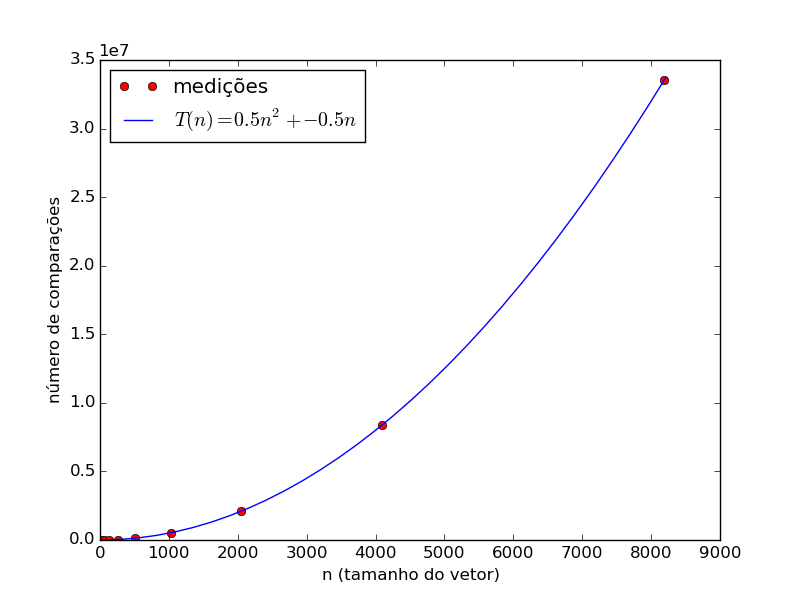
\includegraphics[scale=0.8]{../bolha/imagens/bolhaAleatorio1.png}
\caption{A análise em número de comparações do grafico para $2^{32}$ segue abaixo para bobblesort de vetor aleatório.\\
Tendo a função $T(n) = 0.5*n^2 - 0.5*n$ e para o $n =2^{32}$, $T(2^{32}) = 8.9884 * 10^{307}$}
\label{fig:bolhaAleatorio1}
\end{figure}


\begin{table}[ht]
\centering
\begin{tabular}{rrr} \toprule
        n &    comparações &       tempo(s) \\ \midrule
      32  &            496 &      0.000565 \\
      64  &           2016 &      0.002440 \\
     128  &           8128 &      0.008909 \\
     256  &          32640 &      0.035941 \\
     512  &         130816 &      0.142118 \\
    1024  &         523776 &      0.581946 \\
    2048  &        2096128 &      2.101060 \\
    4096  &        8386560 &      9.395360 \\
    8192  &       33550336 &     36.670900 \\
\bottomrule\addlinespace
\end{tabular}
\caption{Tabela com vetor teste crescente: a linha de interesse analisada para este caso é a 15}
\label{tab:bolhaCrescente}
\end{table}


\begin{figure}[ht]
\centering 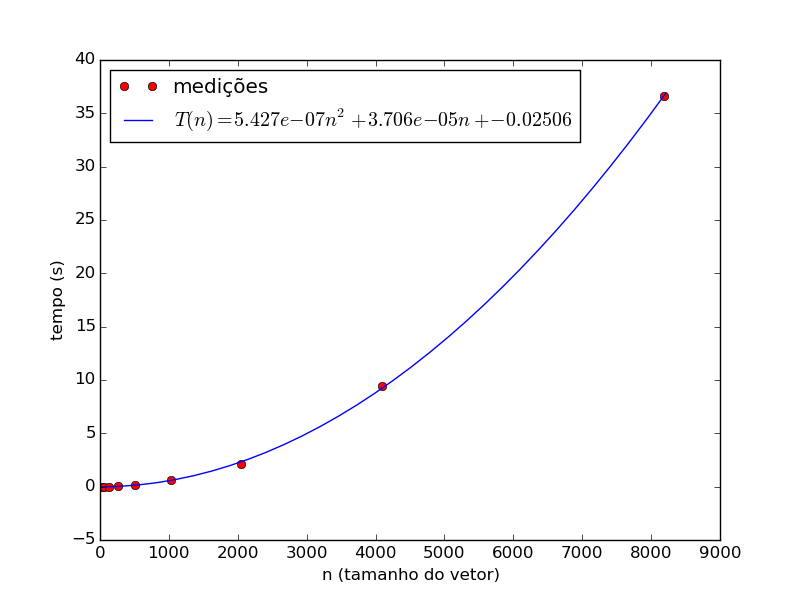
\includegraphics[scale=0.8]{../bolha/imagens/bolhaCrescente0.png}
\caption{A análise do grafico para $2^{32}$ segue abaixo para bubblesort de vetor crescente.\\
Tendo a função $T(n) = 5.427\mathrm{e}-07*n^2+3.706\mathrm{e}-05*n-0.02506$ e para o $n =2^{32}$, $T(2^{32}) = 9.75608 * 10^{301}$}
\label{fig:bolhaCrescente0}
\end{figure}

\begin{figure}[ht]
\centering 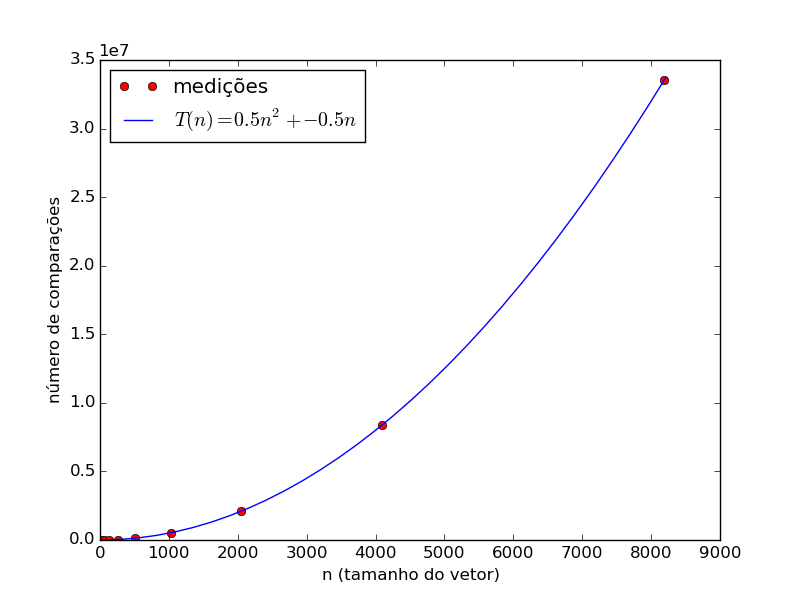
\includegraphics[scale=0.8]{../bolha/imagens/bolhaCrescente1.png}
\caption{A análise em número de comparações do grafico para $2^{32}$ segue abaixo para bobblesort de vetor crescente.\\
Tendo a função $T(n) = 0.5*n^2 - 0.5*n$ e para o $n =2^{32}$, $T(2^{32}) = 8.9884 * 10^{307}$}
\label{fig:bolhaCrescente1}
\end{figure}


\begin{table}[ht]
\centering
\begin{tabular}{rrr} \toprule
        n &    comparações &       tempo(s) \\ \midrule
      32  &            496 &      0.001386 \\
      64  &           2016 &      0.005775 \\
     128  &           8128 &      0.022430 \\
     256  &          32640 &      0.088820 \\
     512  &         130816 &      0.383981 \\
    1024  &         523776 &      1.439680 \\
    2048  &        2096128 &      5.957860 \\
    4096  &        8386560 &     21.605700 \\
    8192  &       33550336 &     93.107000 \\
\bottomrule\addlinespace
\end{tabular}
\caption{Tabela com vetor teste descrescente: a linha de interesse analisada para este caso é a 15}
\label{tab:bolhaDecrescente}
\end{table}


\begin{figure}[ht]
\centering 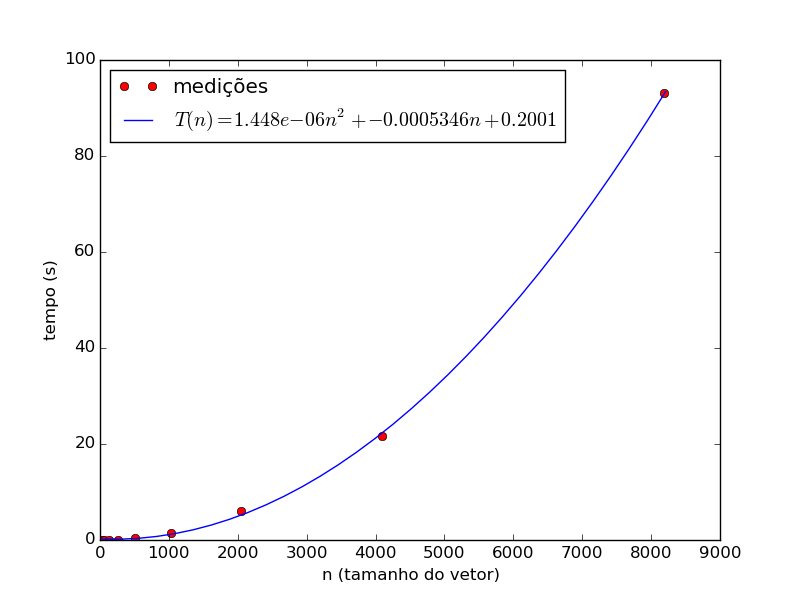
\includegraphics[scale=0.8]{../bolha/imagens/bolhaDecrescente0.png}
\caption{A análise do grafico para $2^{32}$ segue abaixo para bubblesort de vetor decrescente.\\
Tendo a função $T(n) = 9.314\mathrm{e}-07*n^2+0.0001364*n-0.02926$ e para o $n =2^{32}$, $T(2^{32}) = 1.674 * 10^302$}
\label{fig:bolhaDecrescente0}
\end{figure}

\begin{figure}[ht]
\centering 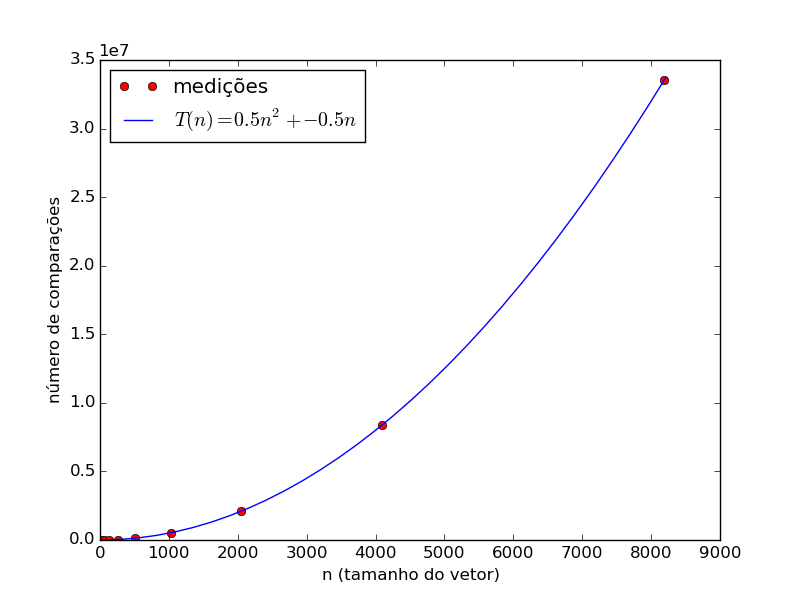
\includegraphics[scale=0.8]{../bolha/imagens/bolhaDecrescente1.png}
\caption{A análise em número de comparações do grafico para $2^{32}$ segue abaixo para bobblesort de vetor decrescente.\\
Tendo a função $T(n) = 0.5*n^2 - 0.5*n$ e para o $n =2^{32}$, $T(2^{32}) = 8.9884 * 10^{307}$}
\label{fig:bolhaDecrescente1}
\end{figure}


\begin{table}[ht]
\centering
\begin{tabular}{rrr} \toprule
        n &    comparações &       tempo(s) \\ \midrule
      32  &            496 &      0.000574 \\
      64  &           2016 &      0.002152 \\
     128  &           8128 &      0.009420 \\
     256  &          32640 &      0.033514 \\
     512  &         130816 &      0.163590 \\
    1024  &         523776 &      0.554991 \\
    2048  &        2096128 &      2.162600 \\
    4096  &        8386560 &      8.656440 \\
    8192  &       33550336 &     35.559200 \\
\bottomrule\addlinespace
\end{tabular}
\caption{Tabela com vetor teste quase crescente 10\%: a linha de interesse analisada para este caso é a 15}
\label{tab:bolhaQuaseCresc10}
\end{table}


\begin{figure}[ht]
\centering 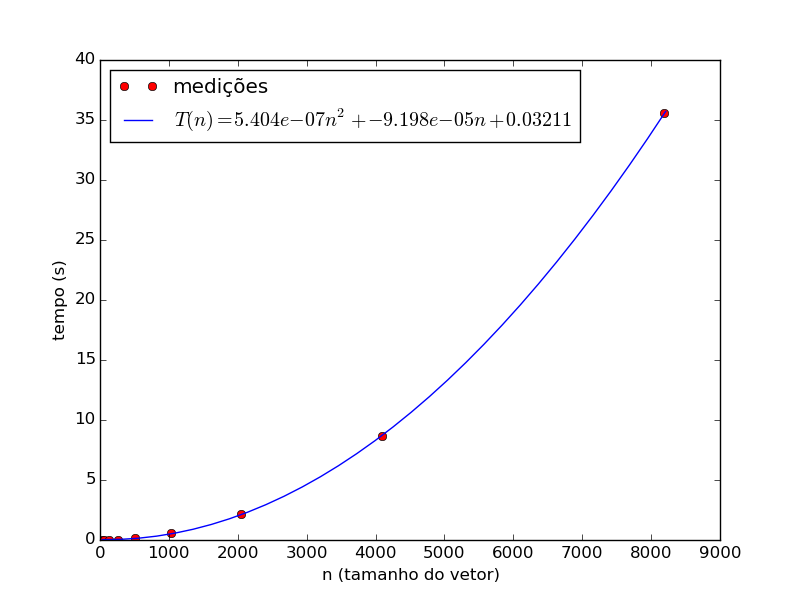
\includegraphics[scale=0.8]{../bolha/imagens/bolhaQuaseCresc100.png}
\caption{A análise do grafico para $2^{32}$ segue abaixo para bubblesort de vetor quase crescente 10\%.\\
Tendo a função $T(n) = 1.226\mathrm{e}-06*n^2+0.0004003*n-0.1198$ e para o $n =2^{32}$, $T(2^{32}) = 2.203 * 10^{302}$}
\label{fig:bolhaQuaseCresc100}
\end{figure}

\begin{figure}[ht]
\centering 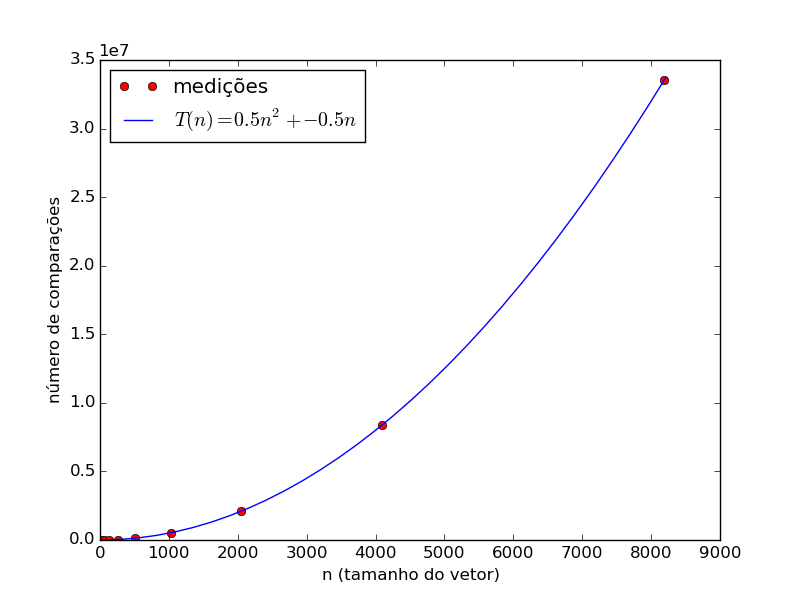
\includegraphics[scale=0.8]{../bolha/imagens/bolhaQuaseCresc101.png}
\caption{A análise em número de comparações do grafico para $2^{32}$ segue abaixo para bobblesort de vetor quase crescente 10\%.\\
Tendo a função $T(n) = 0.5*n^2 - 0.5*n$ e para o $n =2^{32}$, $T(2^{32}) = 8.9884 * 10^{307}$}
\label{fig:bolhaQuaseCresc101}
\end{figure}


\begin{table}[ht]
\centering
\begin{tabular}{rrr} \toprule
        n &    comparações &       tempo(s) \\ \midrule
      32  &            496 &      0.000580 \\
      64  &           2016 &      0.002290 \\
     128  &           8128 &      0.009233 \\
     256  &          32640 &      0.036300 \\
     512  &         130816 &      0.143595 \\
    1024  &         523776 &      0.555577 \\
    2048  &        2096128 &      2.317520 \\
    4096  &        8386560 &      9.365210 \\
    8192  &       33550336 &     39.829700 \\
\bottomrule\addlinespace
\end{tabular}
\caption{Tabela com vetor teste quase crescente 20\%: a linha de interesse analisada para este caso é a 15}
\label{tab:bolhaQuaseCresc20}
\end{table}


\begin{figure}[ht]
\centering 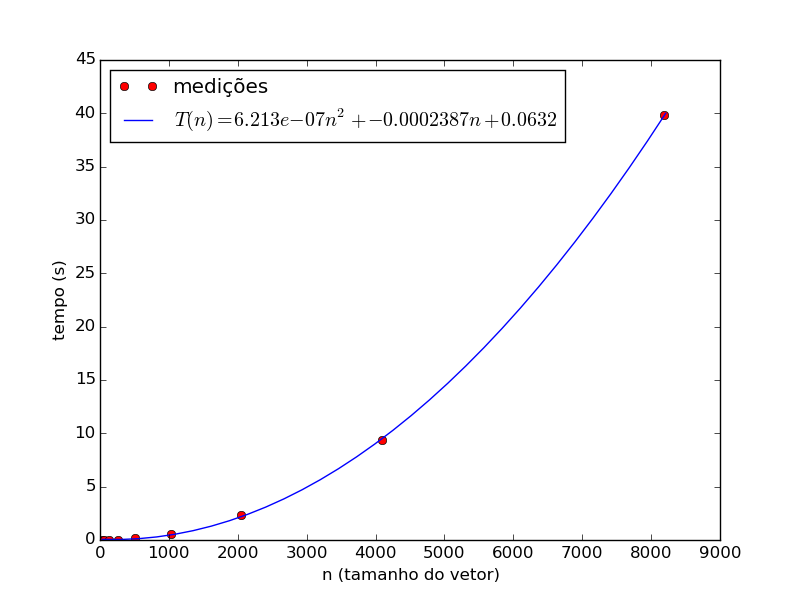
\includegraphics[scale=0.8]{../bolha/imagens/bolhaQuaseCresc200.png}
\caption{A análise do grafico para $2^{32}$ segue abaixo para bubblesort de vetor quase crescente 20\%.\\
Tendo a função $T(n) = 1.639\mathrm{e}-06*n^2+0.001244*n-0.3636$ e para o $n =2^{32}$, $T(2^{32}) = 2.94641 * 10^{302}$}
\label{fig:bolhaQuaseCresc200}
\end{figure}

\begin{figure}[ht]
\centering 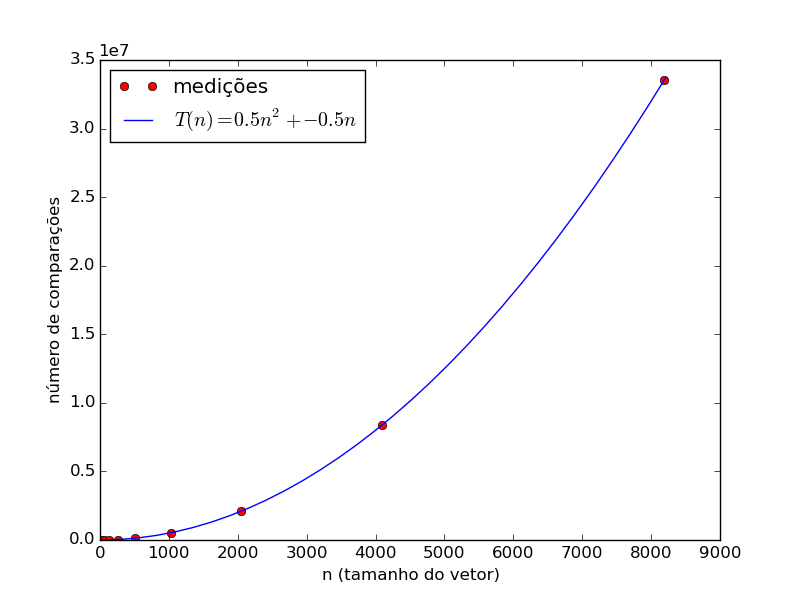
\includegraphics[scale=0.8]{../bolha/imagens/bolhaQuaseCresc201.png}
\caption{A análise em número de comparações do grafico para $2^{32}$ segue abaixo para bobblesort de vetor quase crescente 20\%.\\
Tendo a função $T(n) = 0.5*n^2 - 0.5*n$ e para o $n =2^{32}$, $T(2^{32}) = 8.9884 * 10^{307}$}
\label{fig:bolhaQuaseCresc201}
\end{figure}

\clearpage
\begin{table}[ht]
\centering
\begin{tabular}{rrr} \toprule
        n &    comparações &       tempo(s) \\ \midrule
      32  &            496 &      0.000615 \\
      64  &           2016 &      0.002372 \\
     128  &           8128 &      0.009233 \\
     256  &          32640 &      0.038195 \\
     512  &         130816 &      0.139211 \\
    1024  &         523776 &      0.576390 \\
    2048  &        2096128 &      2.462000 \\
    4096  &        8386560 &      9.317330 \\
    8192  &       33550336 &     37.718900 \\
\bottomrule\addlinespace
\end{tabular}
\caption{Tabela com vetor teste quase crescente 30\%: a linha de interesse analisada para este caso é a 15}
\label{tab:bolhaQuaseCresc30}
\end{table}


\begin{figure}[ht]
\centering 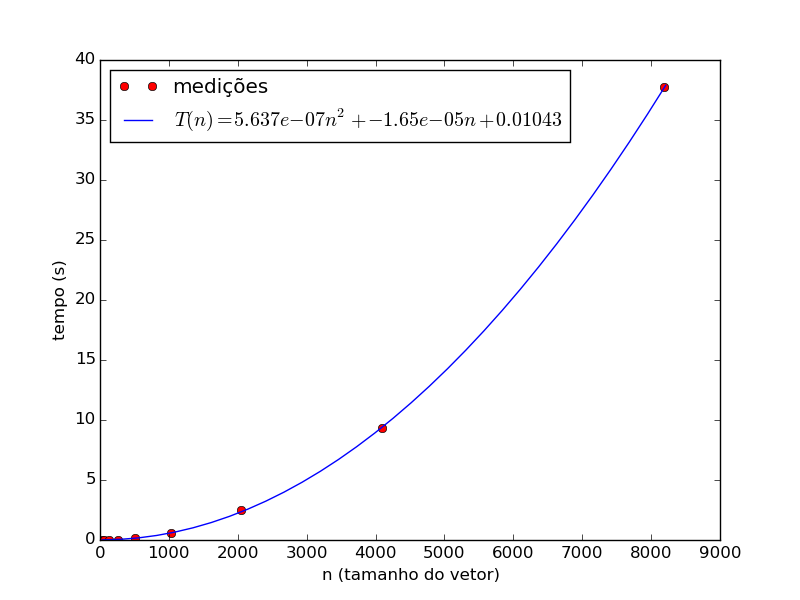
\includegraphics[scale=0.8]{../bolha/imagens/bolhaQuaseCresc300.png}
\caption{A análise do grafico para $2^{32}$ segue abaixo para bubblesort de vetor quase crescente 30\%.\\
Tendo a função $T(n) = 1.305\mathrm{e}-06*n^2+0.0002128*n-0.08068$ e para o $n =2^{32}$, $T(2^{32}) = 2.345989 * 10^{302}$}
\label{fig:bolhaQuaseCresc300}
\end{figure}

\begin{figure}[ht]
\centering 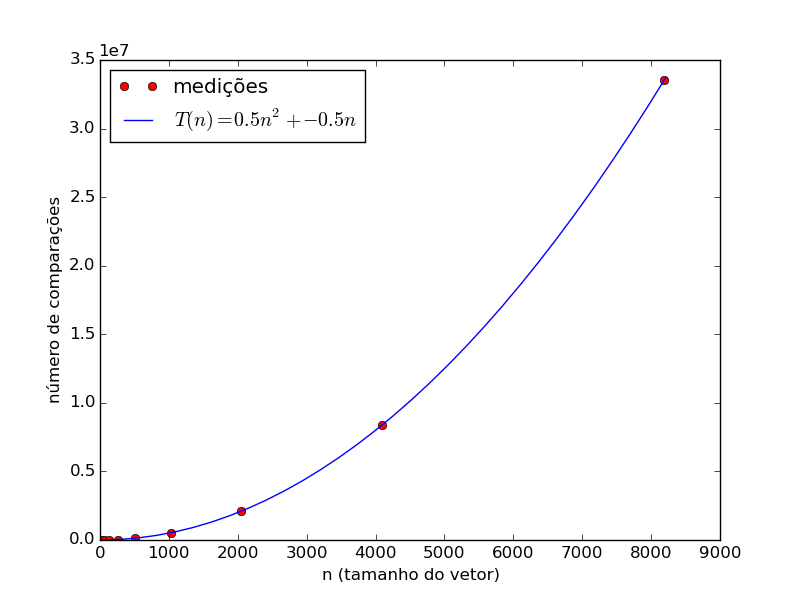
\includegraphics[scale=0.8]{../bolha/imagens/bolhaQuaseCresc301.png}
\caption{A análise em número de comparações do grafico para $2^{32}$ segue abaixo para bobblesort de vetor quase crescente 30\%.\\
Tendo a função $T(n) = 0.5*n^2 - 0.5*n$ e para o $n =2^{32}$, $T(2^{32}) = 8.9884 * 10^{307}$}
\label{fig:bolhaQuaseCresc301}
\end{figure}


\begin{table}[ht]
\centering
\begin{tabular}{rrr} \toprule
        n &    comparações &       tempo(s) \\ \midrule
      32  &            496 &      0.000651 \\
      64  &           2016 &      0.002434 \\
     128  &           8128 &      0.009483 \\
     256  &          32640 &      0.039904 \\
     512  &         130816 &      0.153980 \\
    1024  &         523776 &      0.590784 \\
    2048  &        2096128 &      2.576600 \\
    4096  &        8386560 &      9.910330 \\
    8192  &       33550336 &     41.825800 \\
\bottomrule\addlinespace
\end{tabular}
\caption{Tabela com vetor teste quase crescente 40\%: a linha de interesse analisada para este caso é a 15}
\label{tab:bolhaQuaseCresc40}
\end{table}


\begin{figure}[ht]
\centering 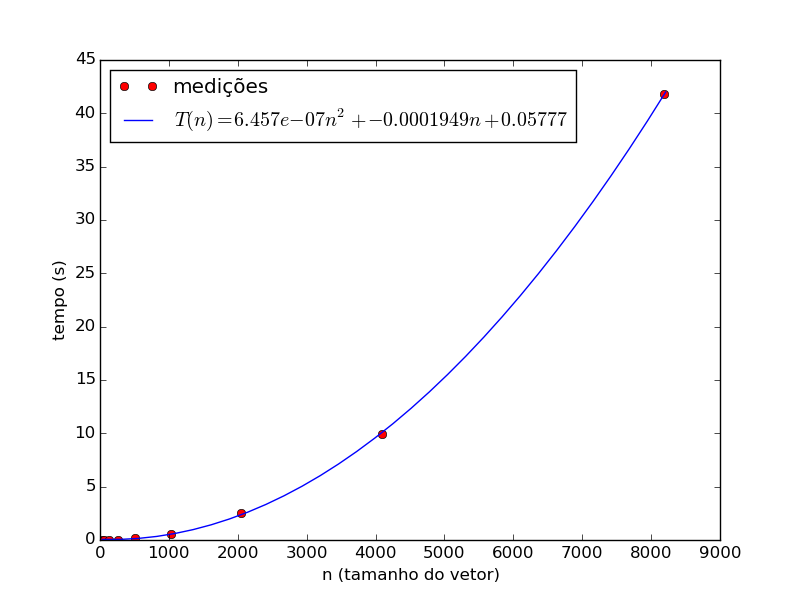
\includegraphics[scale=0.8]{../bolha/imagens/bolhaQuaseCresc400.png}
\caption{A análise do grafico para $2^{32}$ segue abaixo para bubblesort de vetor quase crescente 40\%.\\
Tendo a função $T(n) = 1.425\mathrm{e}-06*n^2+0.0004043*n-0.09253$ e para o $n =2^{32}$, $T(2^{32}) = 2.56171 * 10^{302}$}
\label{fig:bolhaQuaseCresc400}
\end{figure}

\begin{figure}[ht]
\centering 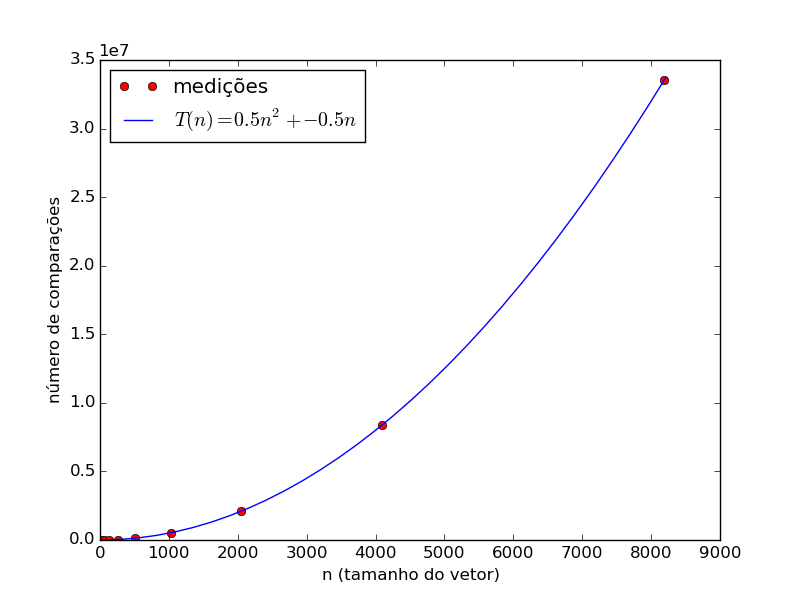
\includegraphics[scale=0.8]{../bolha/imagens/bolhaQuaseCresc401.png}
\caption{A análise em número de comparações do grafico para $2^{32}$ segue abaixo para bobblesort de vetor quase crescente 40\%.\\
Tendo a função $T(n) = 0.5*n^2 - 0.5*n$ e para o $n =2^{32}$, $T(2^{32}) = 8.9884 * 10^{307}$}
\label{fig:bolhaQuaseCresc401}
\end{figure}


\begin{table}[ht]
\centering
\begin{tabular}{rrr} \toprule
        n &    comparações &       tempo(s) \\ \midrule
      32  &            496 &      0.000688 \\
      64  &           2016 &      0.002680 \\
     128  &           8128 &      0.010606 \\
     256  &          32640 &      0.040952 \\
     512  &         130816 &      0.159769 \\
    1024  &         523776 &      0.623442 \\
    2048  &        2096128 &      2.730170 \\
    4096  &        8386560 &     10.305700 \\
    8192  &       33550336 &     38.857700 \\
\bottomrule\addlinespace
\end{tabular}
\caption{Tabela com vetor teste quase crescente 50\%: a linha de interesse analisada para este caso é a 15}
\label{tab:bolhaQuaseCresc50}
\end{table}


\begin{figure}[ht]
\centering 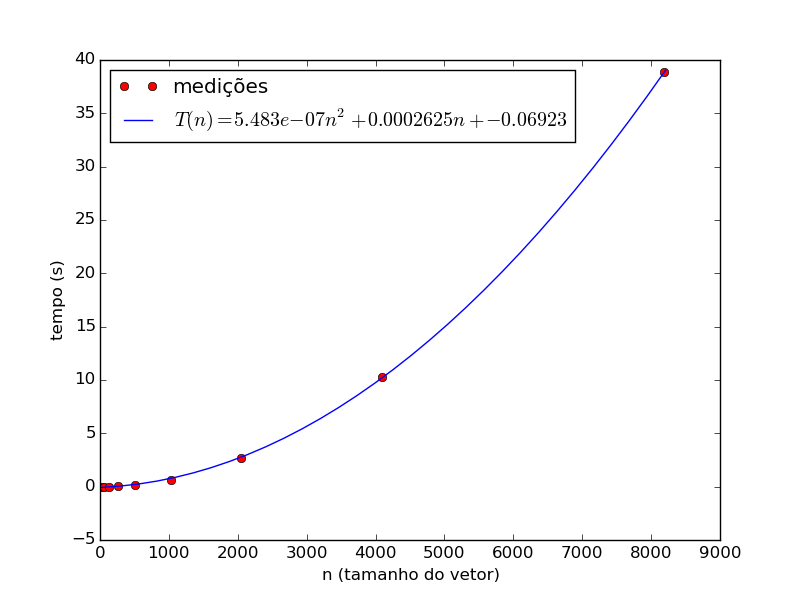
\includegraphics[scale=0.8]{../bolha/imagens/bolhaQuaseCresc500.png}
\caption{A análise do grafico para $2^{32}$ segue abaixo para bubblesort de vetor quase crescente 50\%.\\
Tendo a função $T(n) = 1.211\mathrm{e}-06*n^2+0.0003953*n-0.1445$ e para o $n =2^{32}$, $T(2^{32}) = 2.177006 * 10^{302}$}
\label{fig:bolhaQuaseCresc500}
\end{figure}

\begin{figure}[ht]
\centering 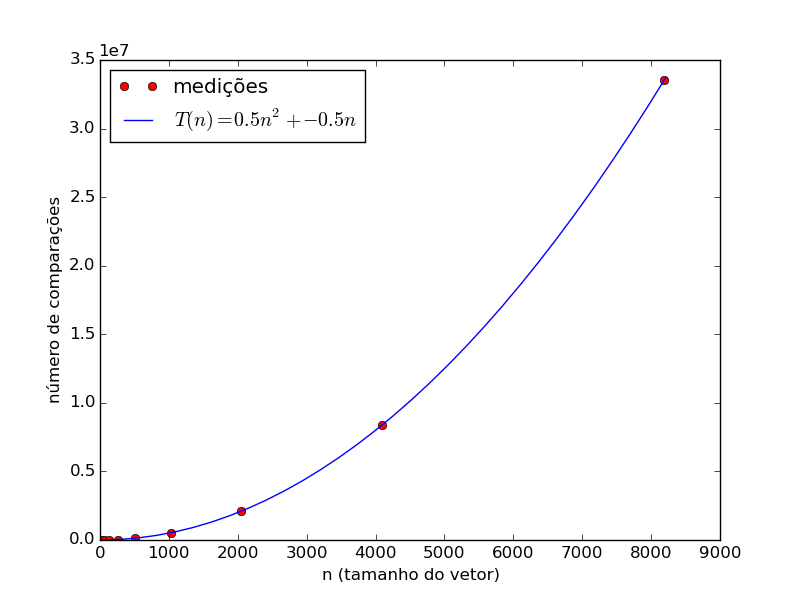
\includegraphics[scale=0.8]{../bolha/imagens/bolhaQuaseCresc501.png}
\caption{A análise em número de comparações do grafico para $2^{32}$ segue abaixo para bobblesort de vetor quase crescente 50\%.\\
Tendo a função $T(n) = 0.5*n^2 - 0.5*n$ e para o $n =2^{32}$, $T(2^{32}) = 8.9884 * 10^{307}$}
\label{fig:bolhaQuaseCresc501}
\end{figure}


\begin{table}[ht]
\centering
\begin{tabular}{rrr} \toprule
        n &    comparações &       tempo(s) \\ \midrule
      32  &            496 &      0.001340 \\
      64  &           2016 &      0.005808 \\
     128  &           8128 &      0.020687 \\
     256  &          32640 &      0.085974 \\
     512  &         130816 &      0.372805 \\
    1024  &         523776 &      1.397550 \\
    2048  &        2096128 &      5.467470 \\
    4096  &        8386560 &     22.445300 \\
    8192  &       33550336 &     85.376500 \\
\bottomrule\addlinespace
\end{tabular}
\caption{Tabela com vetor teste quase decrescente 10\%: a linha de interesse analisada para este caso é a 15}
\label{tab:bolhaQuaseDecresc10}
\end{table}


\begin{figure}[ht]
\centering 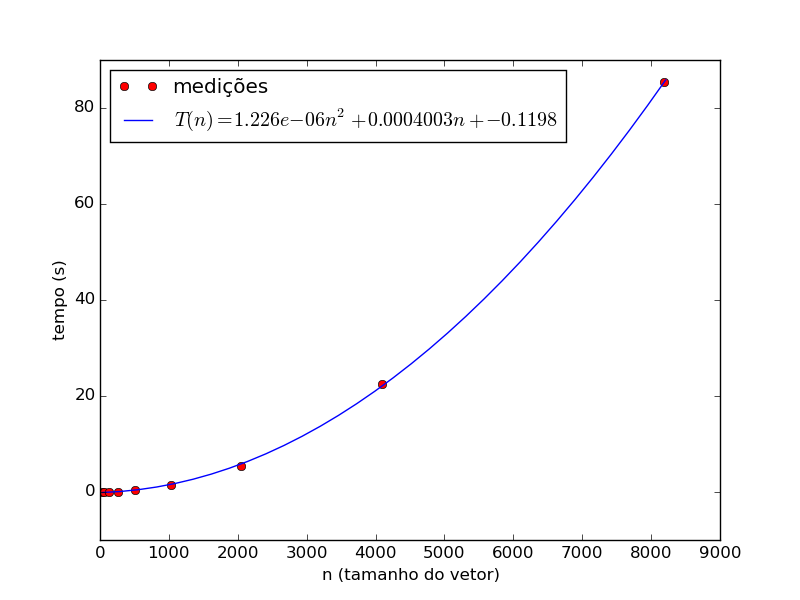
\includegraphics[scale=0.8]{../bolha/imagens/bolhaQuaseDecresc100.png}
\caption{A análise do grafico para $2^{32}$ segue abaixo para bubblesort de vetor quase decrescente 10\%.\\
Tendo a função $T(n) = 5.404\mathrm{e}-07*n^2-\mathrm{e}-05*n-0.03211$ e para o $n =2^{32}$, $T(2^{32}) = 9.71473 * 10^{301}$}
\label{fig:bolhaQuaseDecresc100}
\end{figure}

\begin{figure}[ht]
\centering 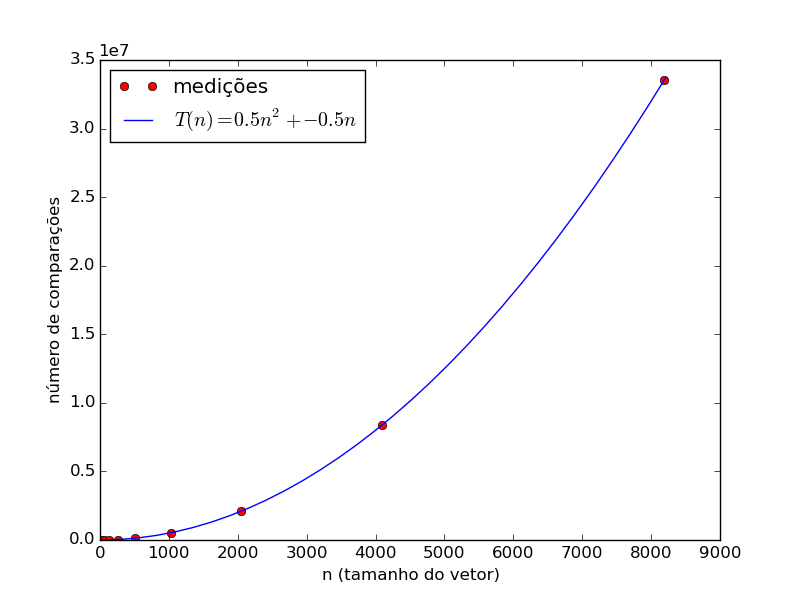
\includegraphics[scale=0.8]{../bolha/imagens/bolhaQuaseDecresc101.png}
\caption{A análise em número de comparações do grafico para $2^{32}$ segue abaixo para bobblesort de vetor quase decrescente 10\%.\\
Tendo a função $T(n) = 0.5*n^2 - 0.5*n$ e para o $n =2^{32}$, $T(2^{32}) = 8.9884 * 10^{307}$}
\label{fig:bolhaQuaseDecresc101}
\end{figure}


\begin{table}[ht]
\centering
\begin{tabular}{rrr} \toprule
        n &    comparações &       tempo(s) \\ \midrule
      32  &            496 &      0.001325 \\
      64  &           2016 &      0.005277 \\
     128  &           8128 &      0.021163 \\
     256  &          32640 &      0.088377 \\
     512  &         130816 &      0.385356 \\
    1024  &         523776 &      1.373970 \\
    2048  &        2096128 &      5.488270 \\
    4096  &        8386560 &     21.906800 \\
    8192  &       33550336 &    100.340000 \\
\bottomrule\addlinespace
\end{tabular}
\caption{Tabela com vetor teste quase decrescente 20\%: a linha de interesse analisada para este caso é a 15}
\label{tab:bolhaQuaseDecresc20}
\end{table}


\begin{figure}[ht]
\centering 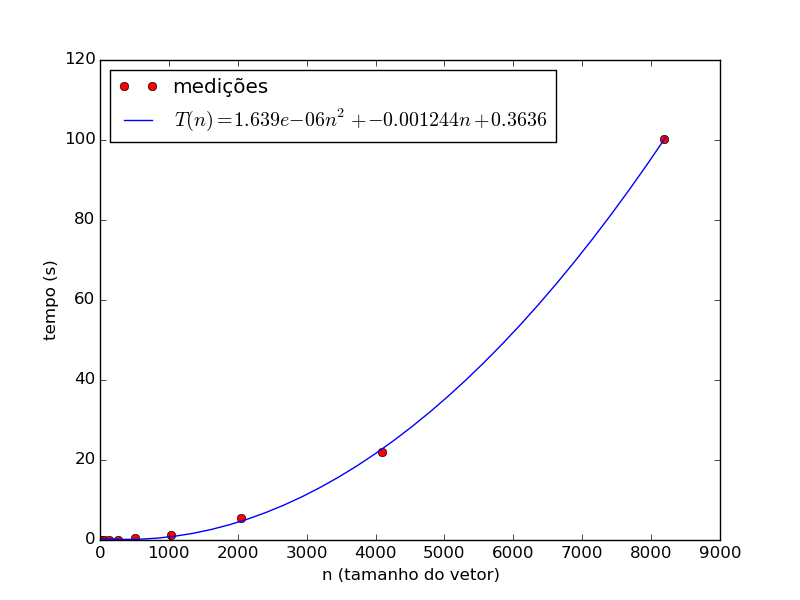
\includegraphics[scale=0.8]{../bolha/imagens/bolhaQuaseDecresc200.png}
\caption{A análise do grafico para $2^{32}$ segue abaixo para bubblesort de vetor quase decrescente 20\%.\\
Tendo a função $T(n) = 5.404\mathrm{e}-07*n^2-\mathrm{e}-05*n-0.0632$ e para o $n =2^{32}$, $T(2^{32}) = 1.116906 * 10^{302}$}
\label{fig:bolhaQuaseDecresc200}
\end{figure}

\begin{figure}[ht]
\centering 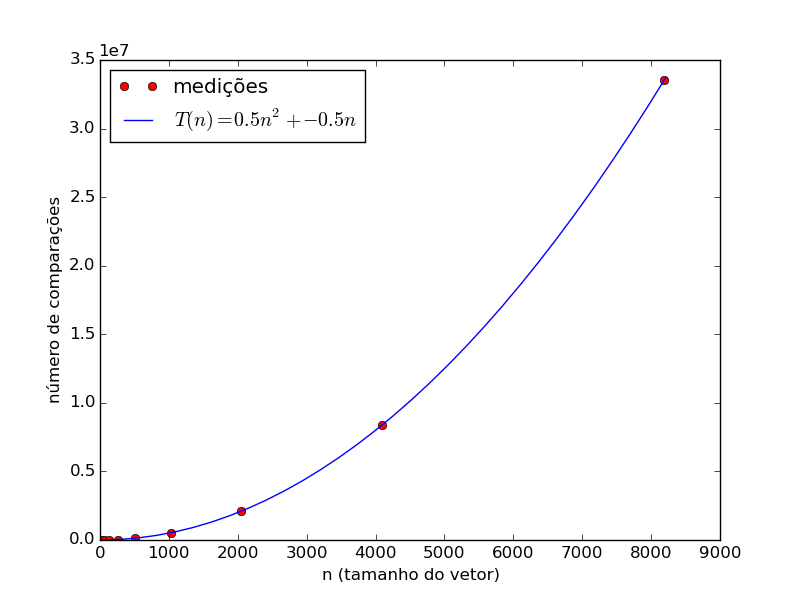
\includegraphics[scale=0.8]{../bolha/imagens/bolhaQuaseDecresc201.png}
\caption{A análise em número de comparações do grafico para $2^{32}$ segue abaixo para bobblesort de vetor quase decrescente 20\%.\\
Tendo a função $T(n) = 0.5*n^2 - 0.5*n$ e para o $n =2^{32}$, $T(2^{32}) = 8.9884 * 10^{307}$}
\label{fig:bolhaQuaseDecresc201}
\end{figure}

\clearpage
\begin{table}[ht]
\centering
\begin{tabular}{rrr} \toprule
        n &    comparações &       tempo(s) \\ \midrule
      32  &            496 &      0.001383 \\
      64  &           2016 &      0.005260 \\
     128  &           8128 &      0.022278 \\
     256  &          32640 &      0.082148 \\
     512  &         130816 &      0.336932 \\
    1024  &         523776 &      1.414750 \\
    2048  &        2096128 &      5.501490 \\
    4096  &        8386560 &     22.978600 \\
    8192  &       33550336 &     89.222100 \\
\bottomrule\addlinespace
\end{tabular}
\caption{Tabela com vetor teste quase decrescente 30\%: a linha de interesse analisada para este caso é a 15}
\label{tab:bolhaQuaseDecresc30}
\end{table}


\begin{figure}[ht]
\centering 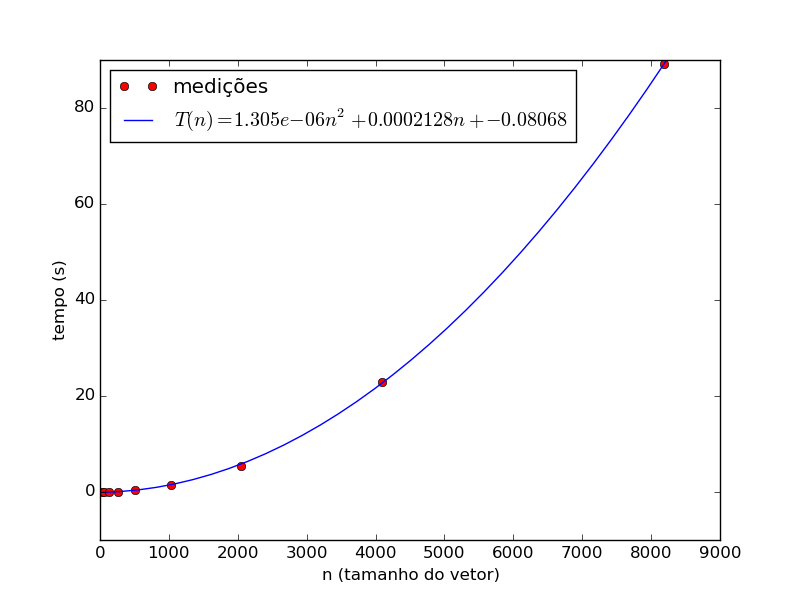
\includegraphics[scale=0.8]{../bolha/imagens/bolhaQuaseDecresc300.png}
\caption{A análise do grafico para $2^{32}$ segue abaixo para bubblesort de vetor quase decrescente 30\%.\\
Tendo a função $T(n) = 5.637\mathrm{e}-07*n^2-1.65\mathrm{e}-5*n-0.01043$ e para o $n =2^{32}$, $T(2^{32}) = 1.0133596 * 10^{302}$}
\label{fig:bolhaQuaseDecresc300}
\end{figure}

\begin{figure}[ht]
\centering 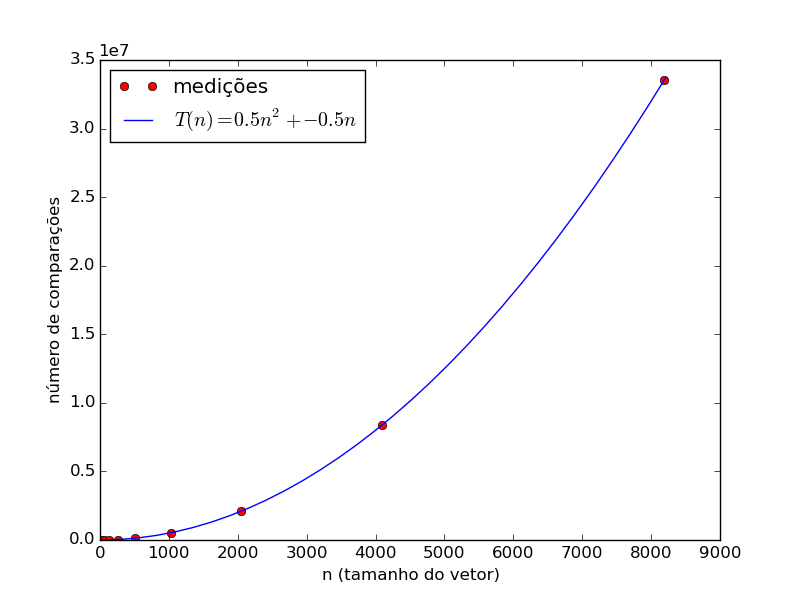
\includegraphics[scale=0.8]{../bolha/imagens/bolhaQuaseDecresc301.png}
\caption{A análise em número de comparações do grafico para $2^{32}$ segue abaixo para bobblesort de vetor quase decrescente 30\%.\\
Tendo a função $T(n) = 0.5*n^2 - 0.5*n$ e para o $n =2^{32}$, $T(2^{32}) = 8.9884 * 10^{307}$}
\label{fig:bolhaQuaseDecresc301}
\end{figure}


\begin{table}[ht]
\centering
\begin{tabular}{rrr} \toprule
        n &    comparações &       tempo(s) \\ \midrule
      32  &            496 &      0.001275 \\
      64  &           2016 &      0.005379 \\
     128  &           8128 &      0.020800 \\
     256  &          32640 &      0.081763 \\
     512  &         130816 &      0.329071 \\
    1024  &         523776 &      1.381690 \\
    2048  &        2096128 &      5.220150 \\
    4096  &        8386560 &     22.260100 \\
    8192  &       33550336 &     92.435900 \\
\bottomrule\addlinespace
\end{tabular}
\caption{Tabela com vetor teste quase decrescente 40\%: a linha de interesse analisada para este caso é a 15}
\label{tab:bolhaQuaseDecresc40}
\end{table}


\begin{figure}[ht]
\centering 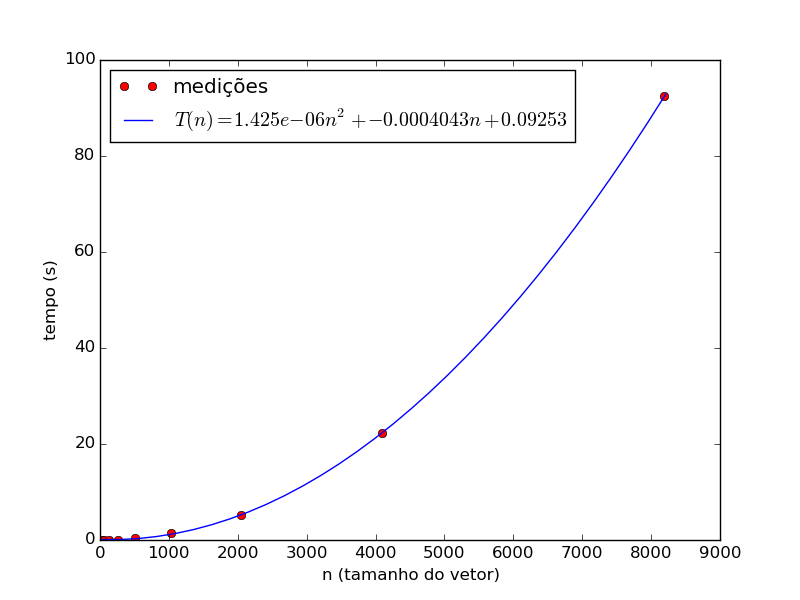
\includegraphics[scale=0.8]{../bolha/imagens/bolhaQuaseDecresc400.png}
\caption{A análise do grafico para $2^{32}$ segue abaixo para bubblesort de vetor quase decrescente 40\%.\\
Tendo a função $T(n) = 6.457\mathrm{e}-07*n^2-0.00019495*n-0.05777$ e para o $n =2^{32}$, $T(2^{32}) = 1.1607704 * 10^{302}$}
\label{fig:bolhaQuaseDecresc400}
\end{figure}

\begin{figure}[ht]
\centering 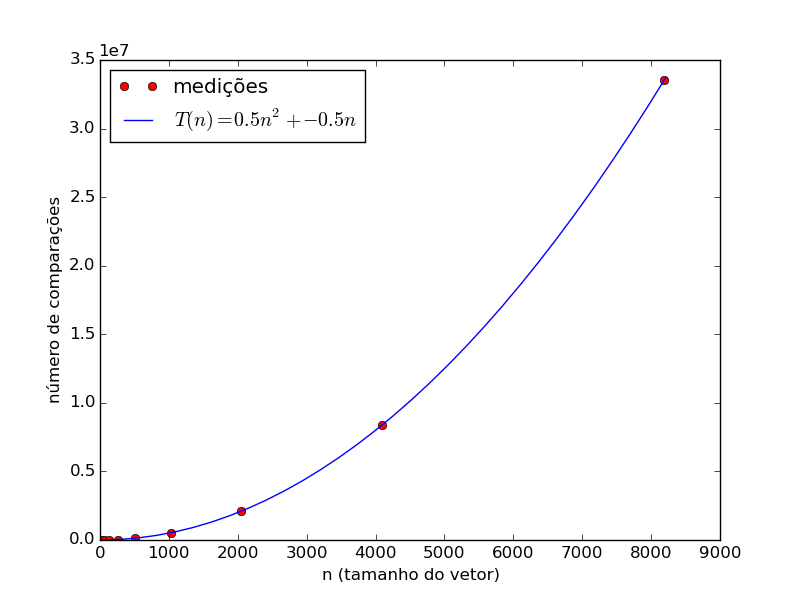
\includegraphics[scale=0.8]{../bolha/imagens/bolhaQuaseDecresc401.png}
\caption{A análise em número de comparações do grafico para $2^{32}$ segue abaixo para bobblesort de vetor quase decrescente 40\%.\\
Tendo a função $T(n) = 0.5*n^2 - 0.5*n$ e para o $n =2^{32}$, $T(2^{32}) = 8.9884 * 10^{307}$}
\label{fig:bolhaQuaseDecresc401}
\end{figure}


\begin{table}[ht]
\centering
\begin{tabular}{rrr} \toprule
        n &    comparações &       tempo(s) \\ \midrule
      32  &            496 &      0.001290 \\
      64  &           2016 &      0.004885 \\
     128  &           8128 &      0.021722 \\
     256  &          32640 &      0.085184 \\
     512  &         130816 &      0.317179 \\
    1024  &         523776 &      1.226130 \\
    2048  &        2096128 &      5.382750 \\
    4096  &        8386560 &     22.192800 \\
    8192  &       33550336 &     84.292500 \\
\bottomrule\addlinespace
\end{tabular}
\caption{Tabela com vetor teste quase decrescente 50\%: a linha de interesse analisada para este caso é a 15}
\label{tab:bolhaQuaseDecresc50}
\end{table}


\begin{figure}[ht]
\centering 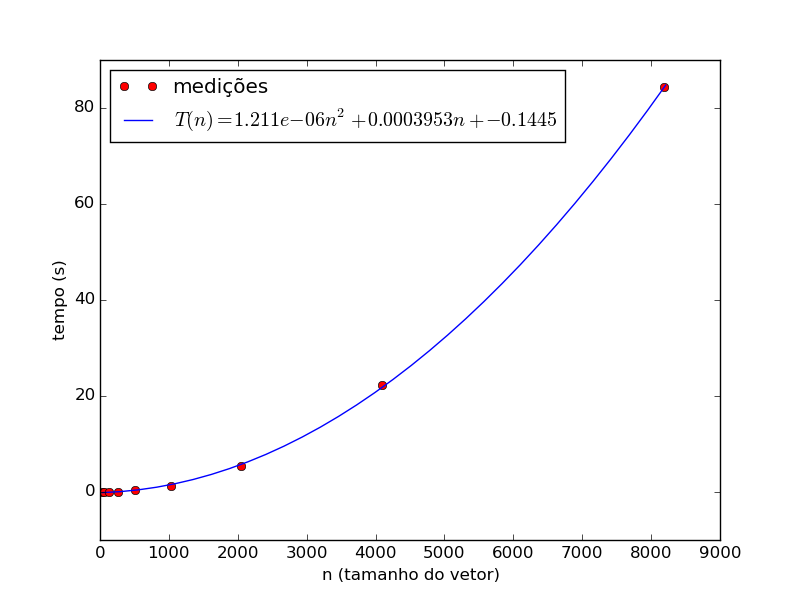
\includegraphics[scale=0.8]{../bolha/imagens/bolhaQuaseDecresc500.png}
\caption{A análise do grafico para $2^{32}$ segue abaixo para bubblesort de vetor quase decrescente 50\%.\\
Tendo a função $T(n) = 5.483\mathrm{e}-07*n^2+0.0002625*n-0.06923$ e para o $n =2^{32}$, $T(2^{32}) = 9.856751 * 10^{301}$}
\label{fig:bolhaQuaseCresc300}
\label{fig:bolhaQuaseDecresc500}
\end{figure}

\begin{figure}[ht]
\centering 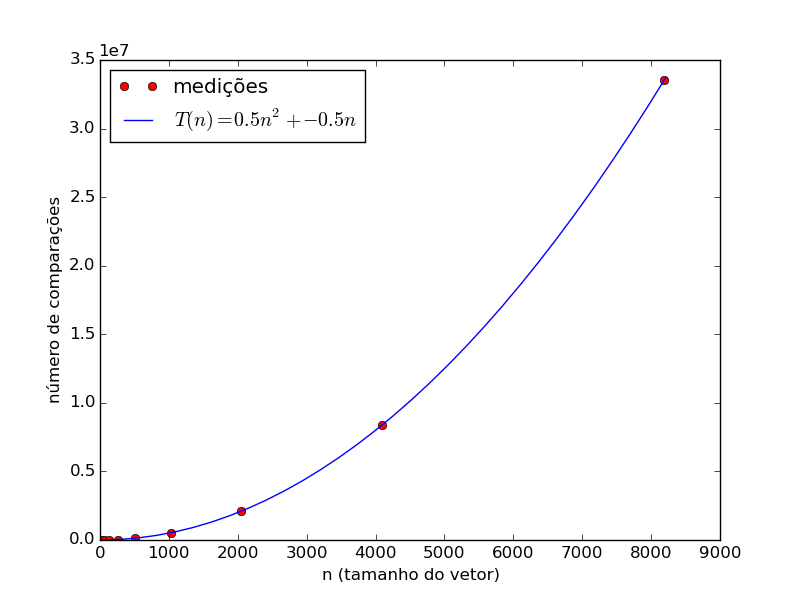
\includegraphics[scale=0.8]{../bolha/imagens/bolhaQuaseDecresc501.png}
\caption{A análise em número de comparações do grafico para $2^{32}$ segue abaixo para bobblesort de vetor quase decrescente 50\%.\\
Tendo a função $T(n) = 0.5*n^2 - 0.5*n$ e para o $n =2^{32}$, $T(2^{32}) = 8.9884 * 10^{307}$}
\label{fig:bolhaQuaseDecresc501}
\end{figure}


\clearpage
\clearpage
\addcontentsline{toc}{part}{Apêndice}
\appendix

\chapter{Arquivo ../bolha/bolha.py \label{ap:bolha}}
\lstinputlisting[caption={../bolha/bolha.py \label{arq:bolha}}]{../bolha/bolha.py}

\chapter{Arquivo ../bolha/ensaio.py \label{ap:bolhaensaio}}
\lstinputlisting[caption={../bolha/ensaio.py \label{arq:bolhaensaio}}]{../bolha/ensaio.py}

\end{document}